\chapter{Anexos}

\section{Diagrama de Casos de Uso}
El diagrama de casos de uso representa las principales interacciones entre el usuario y el sistema AutoSmart. Se muestran las acciones que puede realizar el usuario, como gestionar vehículos, registrar y editar mantenimientos, consultar el historial y configurar notificaciones. El sistema es responsable de enviar notificaciones automáticas cuando corresponde.

% Cuando tengas la imagen, descomenta la línea de abajo:
% \begin{figure}[h!]
%     \centering
%     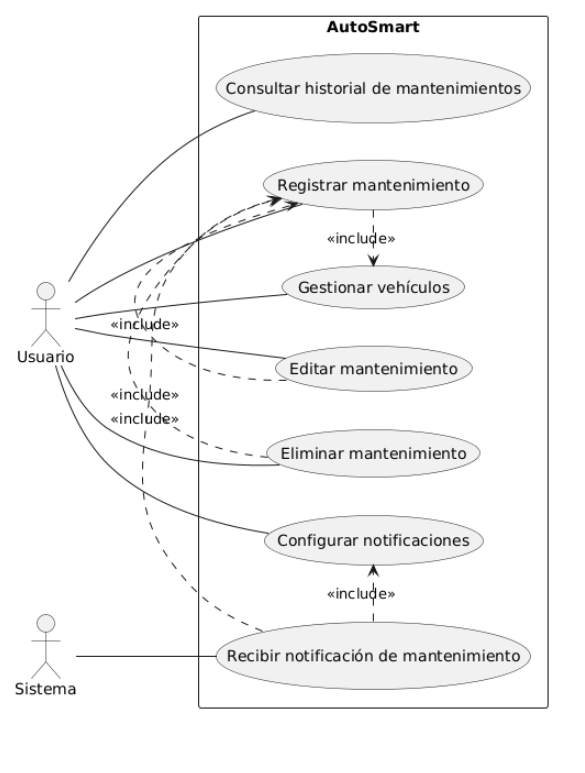
\includegraphics[width=0.8\textwidth]{imagenes/casos_uso.png}
%     \caption{Diagrama de Casos de Uso de AutoSmart}
% \end{figure}

\section{Diagrama Entidad-Relación}
El diagrama entidad-relación muestra la estructura de la base de datos de AutoSmart. Un usuario puede tener varios vehículos, y cada vehículo puede tener varios mantenimientos asociados. Esta estructura permite gestionar de forma eficiente la información y las relaciones entre los datos.

% Cuando tengas la imagen, descomenta la línea de abajo:
% \begin{figure}[h!]
%     \centering
%     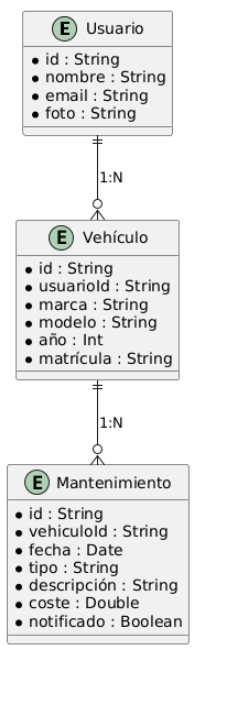
\includegraphics[width=0.8\textwidth]{imagenes/er.png}
%     \caption{Diagrama Entidad-Relación de AutoSmart}
% \end{figure}

\section{Diagrama de Clases}
El diagrama de clases representa la estructura del software a nivel de programación. Se detallan las clases principales: Usuario, Vehículo y Mantenimiento, así como sus atributos y métodos más relevantes. Las relaciones entre clases reflejan la lógica de negocio de la aplicación.

% Cuando tengas la imagen, descomenta la línea de abajo:
% \begin{figure}[h!]
%     \centering
%     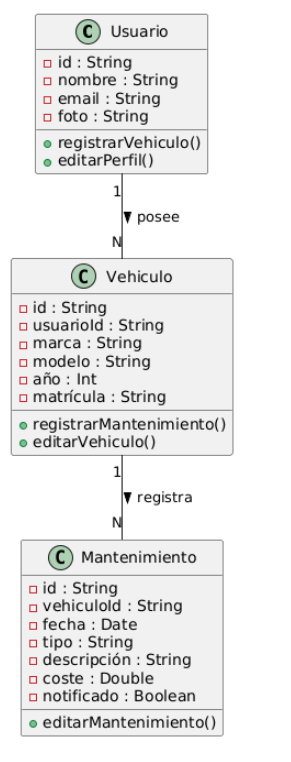
\includegraphics[width=0.8\textwidth]{imagenes/clases.png}
%     \caption{Diagrama de Clases de AutoSmart}
% \end{figure}

\section{Capturas de pantalla}
A continuación se reservan espacios para incluir capturas de pantalla de la aplicación AutoSmart, mostrando las principales pantallas y funcionalidades:

% Ejemplo:
% \begin{figure}[h!]
%     \centering
%     \includegraphics[width=0.7\textwidth]{imagenes/pantalla_inicio.png}
%     \caption{Pantalla de inicio de sesión}
% \end{figure}

% Añade aquí más capturas según lo necesites. 